\rowcolors{2}{\evenRowColor}{\oddRowColor}
\renewcommand{\arraystretch}{1.5}
\begin{longtable}{ C{3cm} C{3cm}  C{3cm}  C{3cm} c }
    \caption{ VAC nei periodi da RR a RP} \\
    \rowcolor{\primaryColor}
    \textcolor{\secondaryColor}{
    \centering\textbf{RR}}     & \textcolor{\secondaryColor}{\centering\textbf{RP}}    & \textcolor{\secondaryColor}
    {\centering\textbf{RQ}} & \textcolor{\secondaryColor}{\centering\textbf{RA}}    \\
    \textit{-}           & 2,86\%                                 & - & - \\
\end{longtable}


\begin{figure}[H]
	\centering
	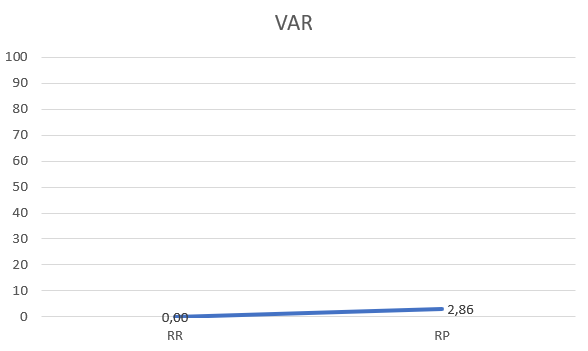
\includegraphics[scale=0.8]{src/ResocontoVerifica/src/img/VAC.png}
	\caption{Variance At Completion durante i periodi da RR a RP}
\end{figure}